\chapter{Nahkampfangriff}
\spp{
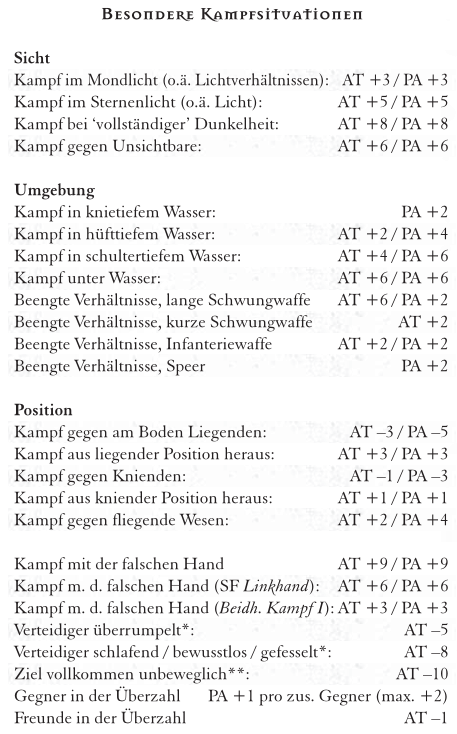
\includegraphics[width=.9\linewidth]{Kampf/Home/kampfsituationen.png}\\
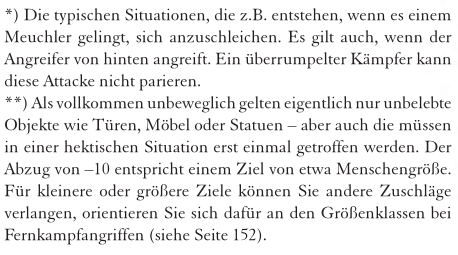
\includegraphics[width=.9\linewidth]{Kampf/Home/kampfsituationenkommentar.png}
}{
\begin{center}
    \begin{tikzpicture}[node distance = 2cm, auto]
            % Nodes
        \node [block] (init) {\hylt{angriff}{angriffstart}{Angriff}} ;
        \node [block, below of=init] (man) {Manöver wählen:\\\hylin{angriffskarten}{NK} / \hylin{fernkampfkarten}{FK}};
        \node [block, below of=man] (erschw) {Erschwernis};
        \node [decision, below =0.3cm of erschw] (par) {\hylt{paradeangr}{parade}{Pariert?}};
        \node [block, below of=par] (end) {\hylin{schaden}{Treffer}};

            % Edges
        \path [line] (init) -> (man);
        \path [line] (man) -> (erschw);
        \path [line] (erschw) -> (par);
        \path [line] (par) -> (end);
    \end{tikzpicture}
\end{center}
\begin{center}
    \begin{tabular}{| c | l |}
        \hline
        \textbf{Zone }& \textbf{Erschwernis}\\
        \hline
        Kopf & +4\\
        \hline
        Brust & +6\\
        \hline
        Arme**& +4/+6\\
        \hline
        Bauch & +4\\
        \hline
        Beine & +2\\
        \hline
    \end{tabular}
\end{center}
\textbf{Gezielter Schlag:} Zonenerschwernis nochmal +2. Kombinierbar mit Finte oder Wuchtschlag

\textbf{Gezielter Stich/Todesstoß auf Zone:} halbe Zonenerschwernis.}
Die \textbf{zweite Angriffsaktion} (umgewandelt) findet \textbf{8} Initiativepunkte \textbf{nach} der Initiative des Akteurs statt.
\textbf{Ansage:} Freiwillige \underline{\textit{plus}} geforderte Erschwernis.
Misslingen: \textbf{nächste} Aktion um gesamte \textbf{Ansage} erschwert.

\chapter{Fernkampfangriff}
\section{Ablauf}
\spp{
\begin{center}
    \begin{tikzpicture}[node distance = 3cm, auto]
            % Nodes
        \node [cloud] (init) {\hypertarget{fernkampf}{\textbf{FK} Angriff (Waffe rdy)}} ;
        \node [decision, below of=init] (atk) {Schnell.?};
        \node [block, below left of=atk] (ssja) {Erschw. +2 (+0 Meist. schütz.)};
        \node [decision, below = 2cm of atk] (ssno) {Zielen / Ansage / Schießen?};
        \node [block, below right of=ssno] (ans) {+1 Akt / 2 Ansagepkt.*};
        \node [block, below left of=ssno] (ziel) {Erschw. -1(max 4) / 2 Akt.};
        \node [block, below of=ans] (ansdmg) {TP + Ansagepkt./2**};
        \node [block, below = 6cm of ssja] (schuss) {Erschw. nach Tabelle***};
            % Edges
        \path [line] (init) -- (atk);
        \path [line] (atk) -- node[above left] {Ja} (ssja);
        \path [line] (atk) -- node {Nein} (ssno);
        \path [line] (ssno) -- node[above left] {Zielen} (ziel);
        \path [line] (ssno) -- node {Ansage} (ans);
        \path [line] (ziel) -- (schuss);
        \path [line] (ans) -- (ansdmg);
        \path [line] (ansdmg) -- (schuss);
        \path [line] (ssja) to[out=230, in=135] (schuss);
        \draw [line] (ssno) to[out=270,in=45] (schuss) ;
    \end{tikzpicture}
\end{center}
\begin{center}
    \begin{tabularx}{\linewidth}{cX}
        \hline
        \textbf{*)} & Ansage <=TaW; Meisterschütze: <= \textbf{FK}\\
        \hline
        \textbf{**)} & \textit{Scharfschütze} darf ganze Ansage addieren. 2 Akt. weniger, mind. 1. \textit{Meisterschütze} immer nur 1 Akt.\\
        \hline
        \textbf{***)} & Dauert Ladezeit+\textit{Schuss} Aktion. Ansage erhöht
        Ladezeit. Schnellschuss: Ladezeit-1 + Schuss. Schnellschuss +
        Gezielter Schuss nicht möglich. Schnellschuss + Schnellladen sind
        kombinierbar.\\
        \hline
    \end{tabularx}
\end{center}
}{
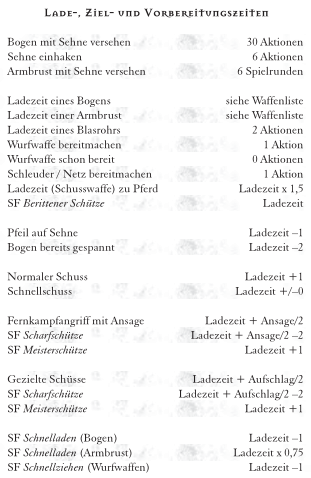
\includegraphics[width=.9\linewidth]{Kampf/Angriff/ladezeiten.png}
}
\section{Erschwernistabelle}
\begin{figure}[H]
    \centering
    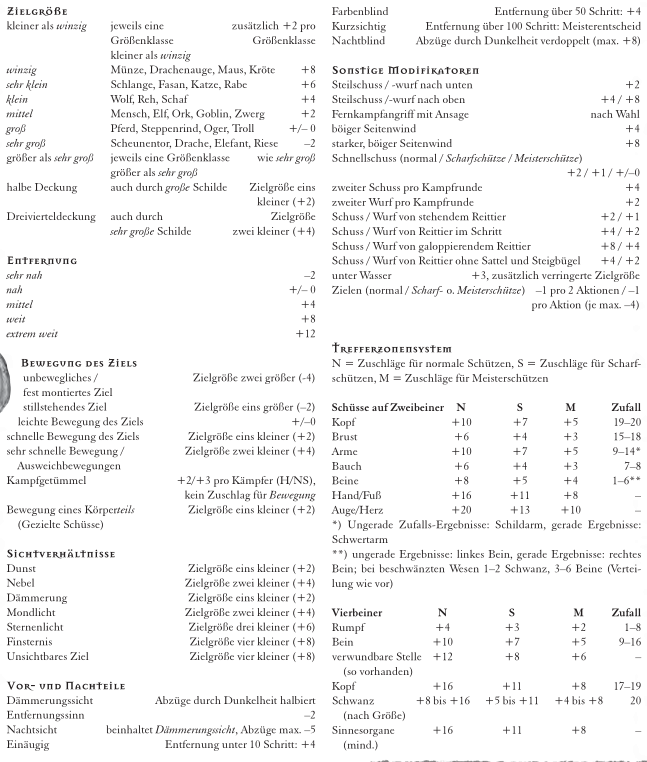
\includegraphics[width=.9\linewidth]{Kampf/Angriff/erschwernisse.png}
\end{figure}